\subsubsection{求解与结果分析：合成回收与相位歧义}

色散相位已经解释条纹位置，本节进一步回答这条关系能否把厚度回收到正确分支，并把合成条件、真实光谱和方法边界分开。求解时以双角联合的两束界面场为主线，峰序与连续相位只承担结构核对。

在生成机制与反演机制一致的共同合成情景中，双束界面场反演的平均绝对相对误差为$0.0008\%$，同一输入下的常折射率峰距基线为$2.59\%$。在相同合成输入上，双束界面场反演的厚度回收误差低于常折射率峰距基线。
% src:求解/问题1/结果/合成验证.json:主指标.数值;常折射率峰距基线.平均绝对相对误差_百分比

因为这里要检验厚度反演本身，正式双束复算把膜层与衬底的折射率、消光系数及偏振权重固定为给定情景，只估计两角共享的厚度。联合损失就是模型反射率与观测反射率之差的平方在两角全部采样点上取平均，比较对象是反射率，而非电场或相位。每角按均匀索引向下取整选取$256$个原始波数坐标，厚度在$0.5$--$40\ \mu\mathrm{m}$内搜索；这个范围是算法搜索域，不是由观测推得的概率区间。
% src:数据/问题1_冻结合成输入/合成设计.json:坐标来源.使用点数_每角
% src:交接/算法参数核对_G4.json:问题一.厚度搜索范围_微米
% src:交接/假设台账_问题1.json:2.假设;3.假设
% 依据:交接/建模笔记_问题1.md:第5节“厚度反演与验证方案”

粗扫先比较$129$个等距厚度点，再对损失最低的$4$个候选作黄金分割精化，逐步缩小候选附近区间，最后取损失最小者。合成真厚度仅参与光谱生成和误差评分，搜索过程依据观测反射率选择候选。连续相位拟厚沿波数展开条纹相位，由相位变化反推厚度，并与场模型相互核对相位级次。
% src:交接/算法参数核对_G4.json:问题一.粗网格点数;问题一.精化候选数
% 依据:交接/建模笔记_问题1.md:第5节“厚度反演与验证方案”

共同案例全部保留，表\ref{tab:04}分列“原型三路线共同24例”与“正式双束复算共同24例”：案例集相同，配置不同，误差分别计算；破折号表示相应配置下未运行该路线。图中的原型逐例点对应前一行，正式复算的双束误差与常折射率峰距基线则配在后一行。
% src:求解/问题1/结果/合成验证.json:主指标.含义;分组汇总.共同匹配.案例数
% src:求解/问题1/原型结果/路线2.json:口径说明.搜索
% src:交接/实验记录.json:66.尝试;66.决定

逐例复核发现，连续相位路线在一个案例中同时保留了$3.0000\ \mu\mathrm{m}$与$36.8799\ \mu\mathrm{m}$两个候选；这里的相位歧义，是不同厚度都通过了相位拟合的候选筛选。计分采用相位回归残差较小的前一个厚度，另一个候选及歧义标记也保留，因此表中平均误差衡量的是所选主候选的回收程度。依据这项全案例核对，双束界面场被选作主方法，峰序与连续相位继续承担独立对照。
% src:求解/问题1/原型结果/路线3.json:合成逐例.0.求解.近优候选厚度_微米;合成逐例.0.求解.厚度_微米;合成逐例.0.求解.候选.0.相位回归均方根残差_弧度;合成逐例.0.求解.候选.1.相位回归均方根残差_弧度;辅助诊断.有歧义案例数
% src:交接/实验记录.json:66.类别;66.尝试;66.现象;66.决定

\begingroup
\small
\begin{longtable}{>{\centering\arraybackslash}p{0.28\textwidth}>{\centering\arraybackslash}p{0.06\textwidth}>{\centering\arraybackslash}p{0.12\textwidth}>{\centering\arraybackslash}p{0.11\textwidth}>{\centering\arraybackslash}p{0.10\textwidth}>{\centering\arraybackslash}p{0.13\textwidth}}
\caption{三路线与朴素基线的合成厚度误差}\label{tab:04}\\
\toprule
情景 & 例数 & 双束场/\% & 峰序/\% & 相位/\% & 峰距基线/\% \\
\midrule
原型三路线共同 & 24 & 0.0010 & 0.0201 & 0.0041 & -- \\
正式另组共同输入 & 24 & 0.0008 & -- & -- & 2.59 \\
新增匹配 & 16 & 0.0011 & -- & -- & -- \\
模型失配 & 10 & 0.3028 & -- & -- & -- \\
\bottomrule
\end{longtable}
\endgroup
% src:求解/问题1/原型结果/路线1.json:主指标值
% src:求解/问题1/原型结果/路线2.json:主指标值
% src:求解/问题1/原型结果/路线3.json:主指标值
% src:求解/问题1/结果/合成验证.json:分组汇总.共同匹配.案例数;分组汇总.新增匹配.案例数;分组汇总.模型失配.案例数;分组汇总.共同匹配.平均绝对相对误差_百分比;分组汇总.新增匹配.平均绝对相对误差_百分比;分组汇总.模型失配.平均绝对相对误差_百分比;常折射率峰距基线.平均绝对相对误差_百分比

共同案例的低误差并没有延伸到所有生成条件。新增匹配的$16$例扩展了厚度、折射率、色散斜率与曲率、偏振和噪声组合，生成与反演仍使用同一光学关系；其中折射率基值改为$2.8$和$3.1$，噪声标准差最高为$0.0015$（反射率比例）。这组案例检验的是改变参数后能否继续回收厚度。
% src:求解/问题1/结果/合成验证.json:分组汇总.新增匹配.案例数
% src:数据/问题1_冻结合成输入/合成设计.json:新增匹配情景

曲率和包络系数采用统一的波数尺度：把原波数减去$2200\ \mathrm{cm}^{-1}$再除以$1800\ \mathrm{cm}^{-1}$，得到无量纲的归一化波数。
% src:数据/问题1_冻结合成输入/合成设计.json:生成规则.归一化波数

模型失配则指生成光谱包含反演时遗漏或误设的成分。失配组共$10$例，包括遗漏$\pm0.12$的色散曲率、将$0.2$的垂直偏振权重按$0.5$求解等情景，图\ref{fig:08}分区比较参数变化与模型缺项的误差。
% src:求解/问题1/结果/合成验证.json:分组汇总.模型失配.案例数
% src:数据/问题1_冻结合成输入/合成设计.json:失配情景.0.生成曲率;失配情景.6.生成曲率;失配情景.1.生成权重;基础情景.垂直偏振权重
% src:交接/图注素材_2.json:0.图题;0.独有信息

其他失配还包括遗漏系数为$\pm0.05$的线性包络、系数为$0.01$的二次基线、消光系数为$0.002$的吸收，以及生成端含$8$束返回而反演仍按一次返回处理；包络与基线以归一化波数为自变量。部分案例同时改变两项，失配组均值因此反映这一组设定的综合影响。
% src:数据/问题1_冻结合成输入/合成设计.json:失配情景.2.生成增益;失配情景.7.生成增益;失配情景.3.生成基线;失配情景.4.生成消光系数;失配情景.5.生成返回束数;生成规则.归一化波数

\begin{figure}[H]
  \centering
  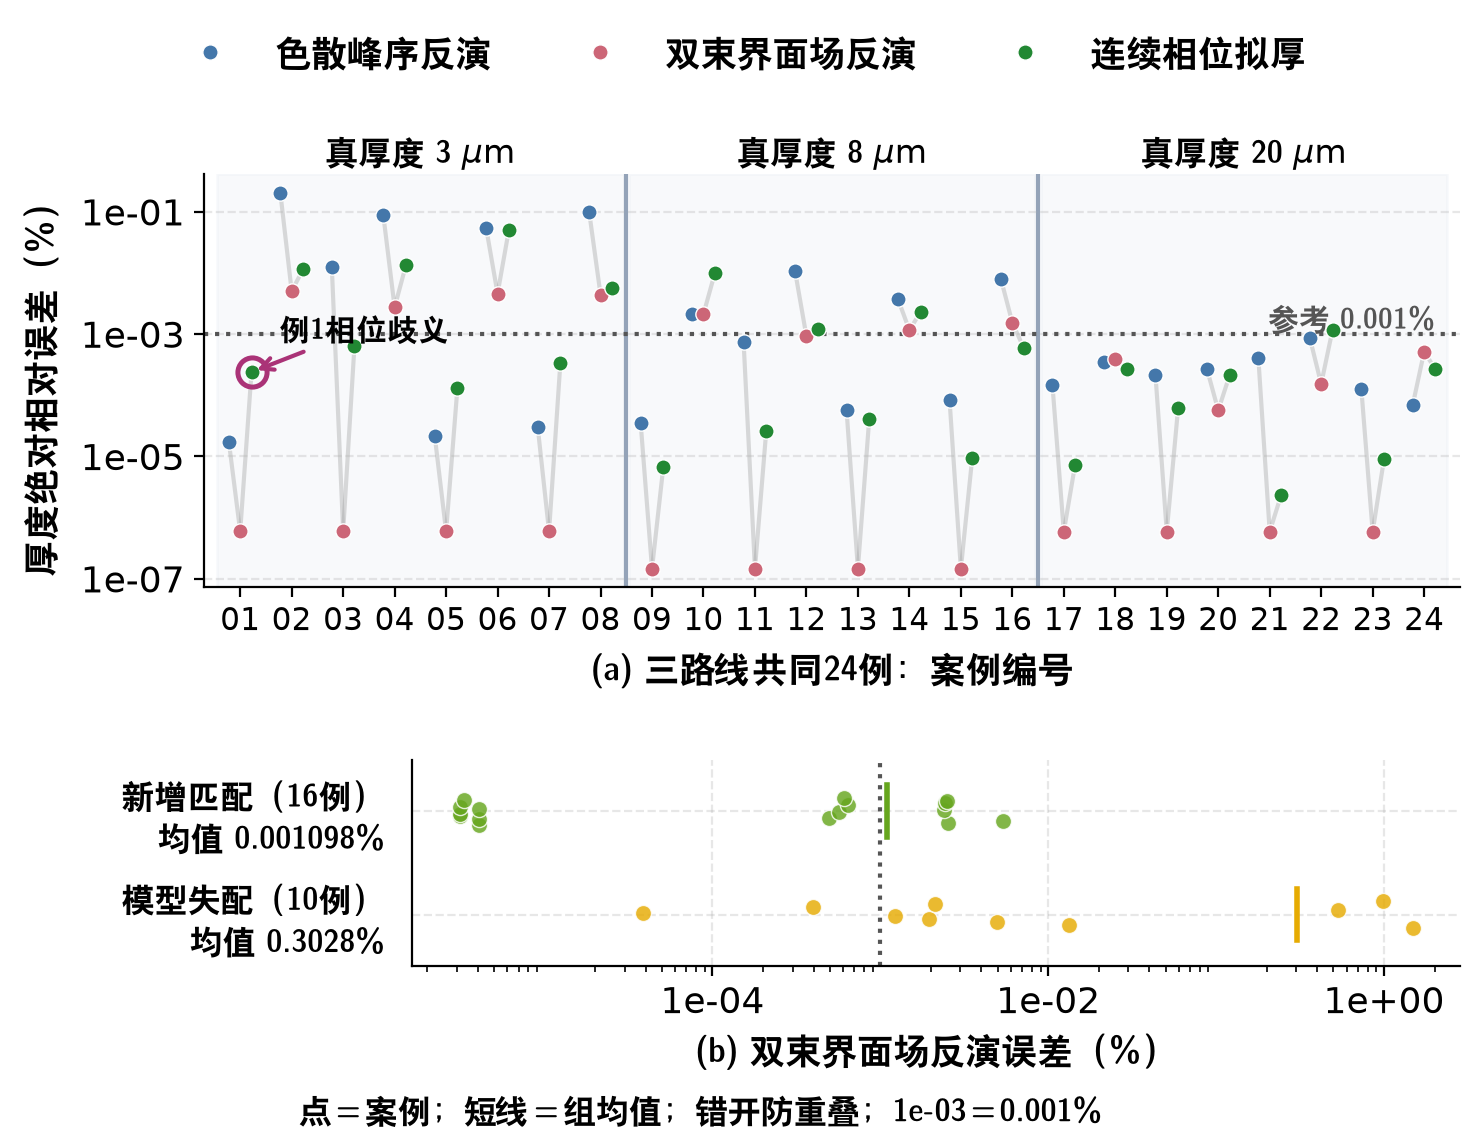
\includegraphics[width=0.96\textwidth]{../求解/问题1/图片/三路线误差按情景分布.png}
  \caption{三路线共同案例与失配情景误差}
  \label{fig:08}
\end{figure}

图\ref{fig:08}下部仅展示主方法在新增匹配与模型失配情景中的误差。上部是原型三路线在共同案例上的逐例配对，对应表\ref{tab:04}的原型行。另将一个角度整谱用于估计厚度，另一个角度整谱用于检验预测，再互换两角，称为两角互换验证；其厚度预测平均绝对相对误差为$0.0018\%$，说明角度互换后的方向性核对与共同案例结论一致。
% src:求解/问题1/结果/独立角度切分验证.json:留出指标.留出厚度预测平均绝对相对误差_百分比;切分原则
% src:交接/图注素材_2.json:0.图题;0.独有信息

保持按$8\ \mu\mathrm{m}$厚度生成的同一组合成观测不变，调整折射率、偏振、平滑宽度和入射角后重估，厚度为$6.66$--$10.01\ \mu\mathrm{m}$。这一厚度重估范围记录同一合成样本对设定变化的响应，比较时固定观测，以分开输入变化与估计条件变化的作用。
% src:数据/问题1_冻结合成输入/合成设计.json:灵敏度锚例.厚度_微米
% src:求解/问题1/结果/灵敏度.json:条件压力范围_微米;范围含义

真实光谱的周期提取先处理缓慢变化的背景。在$2800$--$3600\ \mathrm{cm}^{-1}$窗口内，将反射率与候选周期的正余弦列投影到同一二次基线并取残差，扣除慢变背景后搜索最能解释振荡的周期。
% src:求解/问题1/结果/模型验证.json:真实附件诊断.窗口_每厘米;真实附件诊断.周期投影诊断.0.基线与谐波口径;真实附件诊断.周期投影诊断.1.基线与谐波口径

两谱提取的周期分别为$254.85$和$256.99\ \mathrm{cm}^{-1}$，将两周期的中位数代入定义式得到$T=19.54\ \mu\mathrm{m}$。这里报告的是有限窗口周期统计量；色散和界面相位贡献未被分离，不能直接解释为$dq_1$或几何厚度。式\eqref{eq:period-equivalent}约束的是实际相邻条纹的局部差商，不能把其中的近似条件当作本次窗口拟合已经验证的结论。
% src:求解/问题1/结果/模型验证.json:真实附件诊断.周期_每厘米;真实附件诊断.表观光学厚度乘积_dq_微米

问题一的结论为：双束界面场反演在固定合成条件下的平均回收误差为$0.0008\%$，优于峰距基线的$2.59\%$，实测周期等效量为$T=19.54\ \mu\mathrm{m}$。
% src:求解/问题1/结果/合成验证.json:主指标.数值;常折射率峰距基线.平均绝对相对误差_百分比
% src:求解/问题1/结果/模型验证.json:真实附件诊断.表观光学厚度乘积_dq_微米

本问置信等级为低：周期等效量有独立复算支持，合成回收、常折射率基线比较与两角互换验证支持方法选择。真实附件缺少折射率、消光系数、偏振状态和厚度真值，厚度重估范围较宽，周期等效量尚未换算为标定后的几何厚度。合成误差衡量给定光学条件下的厚度回收，不代表真实晶圆的测量精度。
% src:交接/结果声明_问题1.json:置信.等级;置信.理由

由此，下一问需要利用同片双角的共同信息进一步压缩未知光学因素，把周期等效量推进到可比较的给定光学条件下的厚度。
